\documentclass[11pt]{article}

\usepackage[margin=1in]{geometry}
\usepackage{amsmath,amssymb,amsthm,mathtools}
\newtheorem{proposition}{Proposition}
\usepackage{booktabs}
\usepackage{longtable}
\usepackage{array}
\newcolumntype{L}[1]{>{\raggedright\arraybackslash}p{#1}}
\usepackage{algorithm}
\usepackage{algpseudocode}
\usepackage{listings}
\usepackage{tikz}
\usetikzlibrary{arrows.meta,positioning}
\usepackage{xcolor}
\usepackage{microtype}
\usepackage[hidelinks]{hyperref}
\setlength{\emergencystretch}{3em}
\hbadness=4000

\lstset{
  basicstyle=\ttfamily\footnotesize,
  breaklines=true,
  columns=fullflexible,
  keepspaces=true,
  frame=single,
  framerule=0.3pt,
  xleftmargin=0.4em,
  framexleftmargin=0.4em
}

\DeclareRobustCommand{\code}[1]{\texttt{#1}}
\newcommand{\bfsixteen}{\operatorname{bf16}}
\newcommand{\fpthirtytwo}{\operatorname{fp32}}
\newcommand{\fnuz}{\operatorname{fnuz}}
\newcommand{\rne}{\operatorname{div\_rn}}
\newcommand{\nearby}{\operatorname{nearbyint}}
\newcommand{\MiB}{\,\mathrm{MiB}}
\newcommand{\GiB}{\,\mathrm{GiB}}

\title{A line-level numerical specification of the Terminus Stack~4 trainer\\
on \texttt{gfx942}}
\author{CI-1 production handoff}
\date{13 November 2026}

\begin{document}
\maketitle

\begin{abstract}
The selected trainer is a 24-layer, width-\(2304\) transformer with
\(1{,}446{,}478{,}126\) trainable parameters, a tied vocabulary of
\(65{,}536\), and a \(4096\)-token context. Twenty layers use an inclusive
causal window of \(512\) keys; layers \(6\), \(12\), \(18\), and \(24\) are
global. One sequence therefore contains \(72{,}889{,}344\) valid query--key
pairs. The tensor-core inventory, counting an FMA as two FLOPs and excluding
recompute, is \(9{,}169{,}493{,}760\) FLOPs per token, or
\(1{,}201{,}863{,}886{,}110{,}720\) FLOPs per rank-microstep of
\(M=32\times 4096=131{,}072\) tokens.

The AMD path targets \code{gfx942} (MI300X/MI325X). That device has no
hardware block-scaled MFMA, so every \(128\)-wide FP8 product is scaled in
software inside the \(K\) loop. The operand format is
\code{torch.float8\_e4m3fnuz}, whose finite maximum is \(240\), not the OCP
E4M3 maximum \(448\). A single BF16 residual at the selected microbatch is
\(32\times 4096\times 2304\times 2=603{,}979{,}776\) bytes
(\(576\MiB\)), which exceeds the advertised \(256\,\mathrm{MB}\) last-level
cache, so the kernels stream through HBM. Master weights, gradients, and
optimizer state stay FP32. Hidden matrices use spectral Muon at
\(\eta=0.017\); the tied embedding uses AdamW at \(0.001\). This document
records the arithmetic the source implements. It is not a throughput
measurement, a quality claim, or a statement that a trillion-token run has
been executed.
\end{abstract}

\section{Introduction}

\subsection{What is specified}

The production entry point is \code{production/recipe.py}. Its
\code{SELECTED\_MODEL} fixes the geometry, Peri-LN, learned query/key gains,
learned value residual, BF16 residuals, packed projections, and the streaming
BF16 head. \code{production/amd/recipe.py} copies that geometry and changes
only the linear backend, the attention backend, the split-\(K\) count, and
whether the norm and SwiGLU producers emit an FP8 sidecar. The class defaults
in \code{BitNetLlamaConfig} are a different, smaller model
(\code{vocab\_size}=32{,}000, \code{dim}=768, \code{n\_layers}=20,
\code{local\_attention\_window}=1024, \code{use\_subln}=True). Every number
below is the selected recipe unless a sentence names the class default.

The human-selected dense optimizer, after the 4 November 2026 rate decision,
is spectral Muon \(0.017\), tied-embedding AdamW \(0.001\), ordinary and
Peri-LN norms \(0.0003\), and learned Q/K gains \(0.0001\). The historical
H100 embedding rate \(0.003\) remains in \code{SELECTED\_OPTIMIZER} and is
overridden for AMD dense runs. The QAT table is separate: Muon \(0.0085\),
embedding \(0.003\), norms \(0.00015\), Q/K gains \(0.00005\). The dense
phase sets \code{weight\_mode="dense"}. Ternary codes are the later QAT
phase, not the dense forward.

Token horizon, shard paths, and checkpoints are external to the repository.
The CPU reservation notes describe a \(1\,\mathrm{T}\) main-content budget
and a \(200\,\mathrm{B}\) QAT window; the trainer reads whatever sealed
manifest it is given and refuses a batch that does not divide the manifest.
No measurement in this checkout establishes tokens per second on MI300X or
MI325X, 32-GPU H100 throughput, or dense-to-QAT quality transfer.

\subsection{Hardware constraints that the arithmetic answers}

Three constraints are explicit in the AMD kernels and the configuration note.

\paragraph{No scaled MFMA.}
\code{production/amd/fp8\_kernels.py} states that scales are applied after
each \(128\)-wide reduction tile, and that moving them outside the \(K\) loop
changes the value, because \code{gfx942} has no native scaled MFMA. The
Triton GEMM therefore multiplies the two FP32 scales into the FP32
accumulator on every \(128\)-wide \code{tl.dot}. Deferring that product until
\(K\) is exhausted is a different sum: each partial dot is an FP32 value, and
\((s_a s_b)\sum_t d_t\) equals \(\sum_t (s_a s_b)\,d_t\) only when the scale
is constant across \(t\) \emph{and} the extra multiplies do not change
rounding. The scales \emph{are} constant across a \(128\)-group, but the
implementation multiplies inside the loop so the partials that are actually
summed are the scaled ones. An unscaled FP32 sum followed by one multiply is
rejected by that comment.

\paragraph{The residual does not fit in the last-level cache.}
The selected microbatch stores one BF16 residual of
\(32\times 4096\times 2304\times 2=603{,}979{,}776\) bytes
(\(576\MiB\)), against the advertised \(256\,\mathrm{MB}\) LLC. The
sixteen-sequence residual recorded in \code{CONFIG\_SELECTION.md},
\(301{,}989{,}888\) bytes, is the smaller comparison. The GEMM comment
groups eight \(M\)-tiles so that a weight tile can be reused in that cache.
It does not claim the \(576\MiB\) activation resides there. FP8 codes of one
\(131{,}072\times 2304\) activation are \(288\MiB\); the BF16 tensor the
backward keeps is twice that.

\paragraph{FNUZ saturation at \(240\).}
The quantizer sets \code{FP8} to \code{torch.float8\_e4m3fnuz} and sets
\code{FP8\_MAX} to \code{torch.finfo(FP8).max}. The preflight report string is
``FNUZ E4M3, max 240''. The producer hardcodes the same limit as the literal
\code{240.} The H100 kernels use \code{float8e4nv} and the constant
\(1/448\). The AMD adapter rejects an OCP E4M3 sidecar. Finite quotients are
clamped to \([-\mathrm{FP8\_MAX},\mathrm{FP8\_MAX}]\) before the cast;
nonfinite inputs and nonfinite quotients store NaN.

\subsection{What this paper does not treat as measured}

Native execution of the preflight, the six-tile split-\(K\) search, eight-rank
updates, and checkpoint bandwidth are unrun in this checkout. Where a
quantity is derived from shapes rather than stored as a literal, the
derivation is written out. The dual-layout quantizer loads each
\(128\times 128\) tile once and writes both FNUZ layouts from that FP32 tile.
Column codes use the strided address of the column-only kernel. The selected
\code{balanced} microstep has \(M=131{,}072\) and fused producers on. Its
BF16 quantize reads are \(211.5\GiB\), and the two microsteps of one update
read \(423.0\GiB\). Native timing of the kernel, including whether the
compiler spills the \(64\,\mathrm{KiB}\) tile, is unrun. HBM fit of
microbatch \(32\) is unrun. DDP bucket counts under the
size-greedy rule are \(122\), \(73\), and \(50\) at caps of \(25\), \(64\),
and \(128\MiB\), not \(74\), \(49\), and \(26\).

\section{Model geometry, parameters, and FLOPs}

\subsection{Selected geometry}

\begin{table}[t]
\centering
\caption{Selected fields. Unlisted \code{BitNetLlamaConfig} fields keep the
class default: \code{rms\_norm\_eps}\({}=10^{-5}\),
\code{rope\_theta}\({}=10^{4}\), \code{dropout}\({}=0\),
\code{alpha\_group\_size}\({}=128\), \code{gradient\_checkpointing}\({}=\)false,
\code{ffn\_activation}\({}=\)\code{swiglu}. The class default of
\code{fused\_fp8\_producers} is false; profile \code{balanced} sets it true.}
\label{tab:geom}
\begin{tabular}{@{}ll@{}}
\toprule
Field & Value \\
\midrule
\code{n\_layers}, \code{dim}, \code{ffn\_dim} & \(24\), \(2304\), \(5760\) \\
\code{n\_heads}, \code{n\_kv\_heads}, head dim & \(18\), \(6\), \(2304/18=128\) \\
\code{vocab\_size}, \code{max\_seq\_len} & \(65536\), \(4096\) \\
\code{local\_attention\_window} & \(512\), inclusive of the current token \\
\code{global\_attention\_every} & \(6\) (one-based layers \(6,12,18,24\)) \\
\code{branch\_norm}, \code{use\_subln} & \code{peri}, false \\
\code{qk\_norm\_mode}, \code{value\_residual} & \code{learned\_rms}, \code{learned} \\
\code{residual\_dtype}, \code{residual\_init\_scale} & BF16, \(2^{-2\sqrt{2}}=0.14078571632817444\) \\
\code{weight\_mode}, \code{weight\_init} & \code{dense}, \code{normal} \\
\code{weight\_scale\_layout}, group & \code{blockwise}, \(128\) \\
\code{fp8\_backward}, \code{fp8\_wgrad\_recipe} & \code{full}, \code{1d1d} \\
\code{loss\_backend}, \code{loss\_chunk\_size} & \code{triton}, \(4096\) \\
\code{pad\_token\_id} & \(3\), whose embedding row is zeroed after initialization \\
\bottomrule
\end{tabular}
\end{table}

Head dimension is not stored. It is \code{dim // n\_heads}, and the
constructor rejects a head dimension outside \(\{64,128,256\}\) for any
attention backend other than the reference SDPA path. KV width is
\(6\times 128=768\). Packed QKV output width is
\(2304+2\times 768=3840\). Packed gate/up output width is \(2\times 5760=11520\).

Global layers are the zero-based indices satisfying
\((\ell+1)\bmod 6=0\), that is \(\ell\in\{5,11,17,23\}\). The architecture
note names those layers \(6,12,18,24\). The other twenty layers pass
\code{local\_window}=512. There is no separate \code{lm\_head}. Logits, when
materialized, are \code{F.linear(hidden, tok\_embeddings.weight)}. Training
with \code{return\_logits=False} never forms the full
\([M,65536]\) logit tensor; the streaming loss consumes the tied matrix
directly.

Initialization of every \code{BitLinear} is
\(\mathcal{N}(0,1/\sqrt{d_{\mathrm{in}}})\), then an in-place multiply by
\code{init\_scale}. Output and down projections pass \code{residual=True}, so
that scale is \(2^{-2\sqrt{2}}\). Every other matrix uses scale \(1\). The
embedding is \(\mathcal{N}(0,1/\sqrt{2304})\), and row \(3\) is then zero.
\code{value\_lambda} exists only for \code{layer\_index >= 1} and is
initialized to \((1/2,1/2)\) in FP32. RMSNorm gains are ones. SubLN modules
are \code{nn.Identity} because \code{use\_subln} is false, so the packed
SwiGLU call receives \code{weight=None} and \code{eps=0}.

\subsection{Parameter account}

\code{BitNetLlama.count\_parameters} sums \code{numel} of each parameter. The closed
form in \code{speed\_research/physics.py}, evaluated at 24 layers rather than
that file's 25-layer default, is the asserted total. With
\(W=2304\), \(F=5760\), \(K_{\mathrm{kv}}=768\), \(V=65536\), \(L=24\),
\begin{align*}
P_{\mathrm{proj}}
 &= L\bigl(2W^{2}+2W K_{\mathrm{kv}}+3WF\bigr)
  = 24\times 53{,}968{,}896
  = 1{,}295{,}253{,}504,\\
P_{\mathrm{embed}}
 &= VW = 150{,}994{,}944,\\
P_{\mathrm{small}}
 &= L(4W+2\cdot 128)+W+2(L-1)
  = 227{,}328+2{,}304+46
  = 229{,}678,\\
P
 &= P_{\mathrm{proj}}+P_{\mathrm{embed}}+P_{\mathrm{small}}
  = 1{,}446{,}478{,}126.
\end{align*}
The four channel norms per block are attention input, FFN input, attention
output, and FFN output. The \(2\cdot 128\) term is the shared Q gain and the
shared K gain. The final norm contributes \(W\). The value mix contributes
two scalars in each of the \(23\) layers after layer \(0\).
\code{quantization\_strength} is a buffer, not a parameter. RoPE has no
parameters. Tests assert the total on a meta-device model.

There are \(265\) trainable tensors: ten per layer
(\code{attn\_norm}, \code{ffn\_norm}, \code{attn\_out\_norm},
\code{ffn\_out\_norm}, \code{qkv\_proj}, \code{o\_proj}, \code{q\_norm},
\code{k\_norm}, \code{gate\_up\_proj}, \code{down\_proj}) gives \(240\);
\code{value\_lambda} on layers \(1\) through \(23\) gives \(23\); the
embedding and the final norm give \(2\). Registration order, which is the
order \code{named\_parameters()} and therefore DDP sees before reversal, is
the embedding, then layers \(0\) through \(23\) in the constructor order
above, then the final norm. Inside a layer the constructor order is the four
norms, then attention (lambda if present, QKV, output, Q gain, K gain), then
the FFN (gate/up, down).

\begin{table}[t]
\centering
\caption{Every trainable tensor. Weights are stored \([d_{\mathrm{out}},d_{\mathrm{in}}]\).
FP32 bytes are the master and the gradient. BF16 bytes are the cast used at
a GEMM or residual boundary, not a second master. FP8 bytes are one code
matrix; training also keeps the contiguous transpose of each hidden weight.}
\label{tab:params}
\small
\begin{tabular}{@{}lrrrrr@{}}
\toprule
Tensor & Shape & Copies & Elements & FP32 bytes & FP8 codes \\
\midrule
\code{tok\_embeddings.weight} & \(65536\times 2304\) & 1 & 150{,}994{,}944 & 603{,}979{,}776 & --- \\
\code{qkv\_proj.weight} & \(3840\times 2304\) & 24 & 212{,}336{,}640 & 849{,}346{,}560 & 212{,}336{,}640 \\
\code{o\_proj.weight} & \(2304\times 2304\) & 24 & 127{,}401{,}984 & 509{,}607{,}936 & 127{,}401{,}984 \\
\code{gate\_up\_proj.weight} & \(11520\times 2304\) & 24 & 637{,}009{,}920 & 2{,}548{,}039{,}680 & 637{,}009{,}920 \\
\code{down\_proj.weight} & \(2304\times 5760\) & 24 & 318{,}504{,}960 & 1{,}274{,}019{,}840 & 318{,}504{,}960 \\
\code{attn\_norm.weight} & \(2304\) & 24 & 55{,}296 & 221{,}184 & --- \\
\code{ffn\_norm.weight} & \(2304\) & 24 & 55{,}296 & 221{,}184 & --- \\
\code{attn\_out\_norm.weight} & \(2304\) & 24 & 55{,}296 & 221{,}184 & --- \\
\code{ffn\_out\_norm.weight} & \(2304\) & 24 & 55{,}296 & 221{,}184 & --- \\
\code{q\_norm.weight} & \(128\) & 24 & 3{,}072 & 12{,}288 & --- \\
\code{k\_norm.weight} & \(128\) & 24 & 3{,}072 & 12{,}288 & --- \\
\code{value\_lambda} & \(2\) & 23 & 46 & 184 & --- \\
\code{norm.weight} & \(2304\) & 1 & 2{,}304 & 9{,}216 & --- \\
\midrule
Total & & 265 & 1{,}446{,}478{,}126 & 5{,}785{,}912{,}504 & 1{,}295{,}253{,}504 \\
\bottomrule
\end{tabular}
\end{table}

One FP32 gradient payload is \(1{,}446{,}478{,}126\times 4=5{,}785{,}912{,}504\)
bytes (\(5517.88\MiB\)). Both orientations of the hidden FP8 codes are
\(2\times 1{,}295{,}253{,}504=2{,}590{,}507{,}008\) bytes (\(2.413\GiB\)).
Block scales are one FP32 value per \(128\times 128\) block:
\(1{,}295{,}253{,}504/16384=79{,}056\) scales, and the transpose copy doubles
that to \(632{,}448\) bytes. Those copies are rebuilt when the master
\code{\_version} changes and are dropped in \code{clear\_fp8\_weight\_cache}
after a successful \code{optimizer.step}.

Muon stores one FP32 momentum buffer per hidden matrix,
\(1{,}295{,}253{,}504\times 4=5{,}181{,}014{,}016\) bytes. AdamW stores
\(m\) and \(v\) for the embedding and the \(229{,}678\) small parameters:
\((150{,}994{,}944+229{,}678)\times 8=1{,}209{,}796{,}976\) bytes. Masters,
gradients, Muon momentum, and Adam moments, with no activations and no FP8
cache, are \(17{,}962{,}636{,}000\) bytes (\(16.729\GiB\)).

\subsection{Causal pairs}

A query at position \(t\) (zero-based) may attend to keys \(k\) with
\(0\le t-k < W\) for a local layer, where \(W\) is the inclusive window, and
to all \(k\le t\) for a global layer. The closed form used by
\code{terminus/roofline.py} and \code{speed\_research/physics.py} is
\begin{equation}
C(L,W)=
\begin{cases}
L(L+1)/2 & \text{if the layer is global},\\
W(W+1)/2+(L-W)W & \text{if }W\le L.
\end{cases}
\end{equation}
It equals \(\sum_{t=0}^{L-1}\min(t+1,W)\). At \(L=4096\),
\begin{align*}
C(4096,512)
 &= 512\cdot 513/2+(4096-512)\cdot 512
  = 131{,}328+1{,}835{,}008
  = 1{,}966{,}336,\\
C(4096,\text{global})
 &= 4096\cdot 4097/2
  = 8{,}390{,}656,\\
C_{\mathrm{model}}
 &= 20\cdot 1{,}966{,}336+4\cdot 8{,}390{,}656
  = 72{,}889{,}344.
\end{align*}
The FA3 and ROCm calls do not receive \(512\). They receive
\begin{equation}
\mathrm{window\_size}=
\begin{cases}
(-1,-1) & \text{global layer},\\
(511,0) & \text{local layer}.
\end{cases}
\end{equation}
The left entry \(511\) plus the current key is the inclusive window of
\(512\). The right entry \(0\) forbids future keys. AITER is also passed
\code{how\_v3\_bf16\_cvt=0}. The comment states that the alternative default
on \code{gfx942} is round-to-nearest-away, and that \(0\) selects
round-to-nearest-even so the BF16 conversion matches the PyTorch and FA3
convention more closely. Dropout is \(0\). \code{deterministic=False} is
passed on both the dense and the variable-length calls: the rest of the
trainer fixes rounding and seeds, and this attention flag does not request
the deterministic backward variant.

\subsection{FLOPs per token and per microstep}

\code{operation\_inventory} counts an FMA as two FLOPs and does not count
replay, softmax, norms, or casts. Projection parameters are read three times
in the backward sense (forward, input gradient, weight gradient), and each
read is a multiply-add:
\begin{align*}
F_{\mathrm{FP8}}
 &= 6\,P_{\mathrm{proj}}
  = 7{,}771{,}521{,}024,\\
F_{\mathrm{head}}
 &= 6\,VW
  = 905{,}969{,}664,\\
F_{\mathrm{attn}}
 &= 12\,W\,C_{\mathrm{model}}/L
  = 12\cdot 2304\cdot 72{,}889{,}344/4096
  = 492{,}003{,}072.
\end{align*}
The attention factor \(12\) is QK and PV in the forward plus both operand
gradients of each. The sum is \(9{,}169{,}493{,}760\) FLOPs per token.
At the selected \(M=131{,}072\),
\begin{equation}
M\cdot 9{,}169{,}493{,}760 = 1{,}201{,}863{,}886{,}110{,}720
\end{equation}
FLOPs per rank per microstep on this inventory. The balanced update runs two
such microsteps on each of eight ranks. Each rank still scores \(262{,}144\)
tokens, so one rank's inventory for one update remains
\(2{,}403{,}727{,}772{,}221{,}440\) FLOPs. The H100 roofline adds a
further \(F_{\mathrm{attn}}/2\) BF16 operations for FA3 QK replay when
checkpointing is off. That extra \(82{,}000{,}512\) FLOPs per token is not
in the \(9.1695\times 10^{9}\) figure. The roofline function refuses AMD
backends. Neither inventory is a measured service time. The H100 NVL peaks
hardcoded beside it are \(1671\) TFLOP/s FP8 and \(835.5\) TFLOP/s BF16 in
\code{roofline.py}, and \(1670.5\) TFLOP/s FP8 in \code{physics.py}. Those
constants are not \code{gfx942} rates.

\subsection{Packed projections and logical Muon slices}

The GEMM sees one matrix. Muon does not. \code{logical\_muon\_rows} partitions
rows of \code{qkv\_proj.weight} into \((2304,768,768)\) and rows of
\code{gate\_up\_proj.weight} into \((5760,5760)\). Output and down
projections are one slice each. Momentum is one buffer the size of the
packed parameter; each slice is a view. Newton--Schulz batches slices that
share \((\mathrm{rows},\mathrm{cols},\mathrm{adjust\_lr\_fn})\). At this
width the batches are: all \(24\) query slices with all \(24\) output slices
(\(2304\times 2304\)); all \(48\) key and value slices (\(768\times 2304\));
all \(48\) gate and up slices (\(5760\times 2304\)); all \(24\) down slices
(\(2304\times 5760\)).

The spectral coefficient is \(\sqrt{d_{\mathrm{out}}/d_{\mathrm{in}}}\) on
the raw Newton--Schulz factor, with no \(0.2\), no \(\max(1,\cdot)\), and no
width-growing multiplier. The Python value is \code{(rows/cols)**0.5}.

\begin{table}[t]
\centering
\caption{Logical Muon slices. Six-decimal values match the spectral note.
The step uses the unrounded square root.}
\label{tab:spectral}
\begin{tabular}{@{}lrrl@{}}
\toprule
Slice & \(d_{\mathrm{out}}/d_{\mathrm{in}}\) & \(\sqrt{\cdot}\) & Documented 6 d.p. \\
\midrule
Q, O & \(2304/2304=1\) & \(1\) & \(1\) \\
K, V & \(768/2304=1/3\) & \(0.5773502691896257\) & \(0.577350\) \\
gate, up & \(5760/2304=5/2\) & \(1.5811388300841898\) & \(1.581139\) \\
down & \(2304/5760=2/5\) & \(0.6324555320336759\) & \(0.632456\) \\
\bottomrule
\end{tabular}
\end{table}

The same ratios hold at widths \(768\) and \(1536\) because every hidden
dimension in this family scales together. Decay uses \(\eta\) times \(0.02\)
and does not include the shape factor.

\subsection{One block}

\begin{figure}[t]
\centering
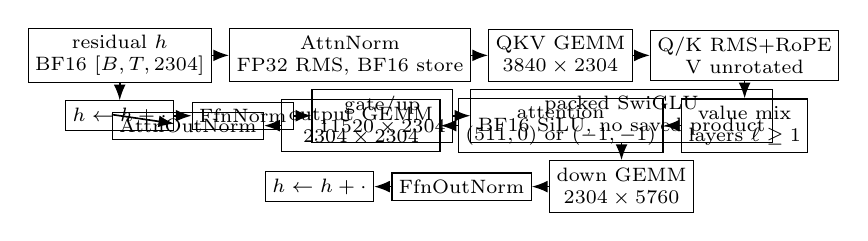
\begin{tikzpicture}[
  node distance=2.2mm,
  box/.style={draw, font=\scriptsize, align=center, inner sep=2.5pt},
  arr/.style={-{Latex}, semithick}
]
\node[box] (h) {residual \(h\)\\BF16 \([B,T,2304]\)};
\node[box, right=of h] (an) {AttnNorm\\FP32 RMS, BF16 store};
\node[box, right=of an] (qkv) {QKV GEMM\\ \(3840\times 2304\)};
\node[box, right=of qkv] (qk) {Q/K RMS+RoPE\\V unrotated};
\node[box, below=of qk] (mix) {value mix\\layers \(\ell\ge 1\)};
\node[box, left=of mix] (attn) {attention\\\((511,0)\) or \((-1,-1)\)};
\node[box, left=of attn] (o) {output GEMM\\ \(2304\times 2304\)};
\node[box, left=of o] (aon) {AttnOutNorm};
\node[box, below=of h] (res1) {\(h \leftarrow h+\cdot\)};
\node[box, right=of res1] (fn) {FfnNorm};
\node[box, right=of fn] (gu) {gate/up\\ \(11520\times 2304\)};
\node[box, right=of gu] (sw) {packed SwiGLU\\BF16 SiLU, no saved product};
\node[box, below=of sw] (dn) {down GEMM\\ \(2304\times 5760\)};
\node[box, left=of dn] (fon) {FfnOutNorm};
\node[box, left=of fon] (res2) {\(h \leftarrow h+\cdot\)};
\draw[arr] (h)--(an);\draw[arr] (an)--(qkv);\draw[arr] (qkv)--(qk);
\draw[arr] (qk)--(mix);\draw[arr] (mix)--(attn);\draw[arr] (attn)--(o);\draw[arr] (o)--(aon);
\draw[arr] (aon)--(res1);\draw[arr] (h.south)--(res1.north);
\draw[arr] (res1)--(fn);\draw[arr] (fn)--(gu);\draw[arr] (gu)--(sw);
\draw[arr] (sw)--(dn);\draw[arr] (dn)--(fon);\draw[arr] (fon)--(res2);
\end{tikzpicture}
\caption{Dataflow of one block with \code{branch\_norm="peri"} and
\code{use\_subln=False}. SubLN would have sat between attention and the
output projection, and between SwiGLU and the down projection. It is an
identity. The value residual reads layer \(0\)'s raw \(V\), not the mixed
\(V\) of layer \(\ell-1\).}
\label{fig:block}
\end{figure}

Peri-LN normalizes the branch input and normalizes again after the branch's
output projection, before the residual add:
\begin{equation}
h \leftarrow h + \mathrm{AttnOutNorm}(\mathrm{Attn}(\mathrm{AttnNorm}(h))),
\qquad
h \leftarrow h + \mathrm{FfnOutNorm}(\mathrm{FFN}(\mathrm{FfnNorm}(h))).
\end{equation}
Each of those four norms is a channel gain of length \(2304\). The next
layer's AttnNorm therefore sees the sum, not the branch output. That sum is
also the tensor whose backward splits into the skip and the branch. The
value-residual edge is not on this sum. It leaves layer \(0\)'s \(V\) and
enters every later layer inside attention, before AttnOutNorm. Fusing
AttnOutNorm, the residual add, and the next AttnNorm into one kernel would
not see \(V_0\), and a checkpoint wrapped around layer \(0\) would store
\(V_0\) without a gradient. The forward comment states the consequence:
layer \(0\)'s value projection would stop learning. The selected recipe
leaves \code{gradient\_checkpointing} false, and the exclusion remains in the
forward for any caller that turns checkpointing on. Later layers may be
checkpointed with \code{use\_reentrant=False}; \(V_0\) is then an input of
those regions, which non-reentrant checkpoint tracks.

\subsection{RMSNorm}

The unfused module computes the norm in FP32 and stores BF16:
\begin{equation}
y = \bfsixteen\!\left(
  x_{\mathrm{fp32}}\cdot
  \left(\mathrm{mean}(x_{\mathrm{fp32}}^{2})+\epsilon\right)^{-1/2}
  \cdot g_{\mathrm{fp32}}
\right),
\end{equation}
with \(\epsilon=10^{-5}\). The Triton forward does the same reduction in
FP32, multiplies the gain in FP32, and casts once to the output dtype. The
launch sets \code{enable\_fp\_fusion=False}, so the compiler is not invited
to contract that cast into the multiply. The FP32 inverse is saved, one
scalar per row. Backward recomputes
\(\hat{x}=x\cdot\mathrm{inverse}\) before the gain, accumulates
\(\mathrm{d}g=\sum \mathrm{d}y\,\hat{x}\), multiplies \(\mathrm{d}y\) by the
gain, and applies the standard RMS Jacobian
\begin{equation}
\mathrm{d}x
 =
 \left(\mathrm{d}y - \hat{x}\cdot\frac{1}{W}\sum_i \mathrm{d}y_i\hat{x}_i\right)
 \cdot\mathrm{inverse},
\end{equation}
stored in the activation dtype. The gain gradient is reduced in FP32 over at
most \(512\) programs when the gain is a channel vector, then cast to the
parameter dtype.

A producer that emits FNUZ does this BF16 store first, then quantizes the
rounded register value. It does not quantize the pre-round FP32 vector. The
preflight requires the resulting codes and scales to be bitwise equal to a
separate \code{quantize(..., eps=1e-5)} of the BF16 tensor.

\subsection{Learned Q/K norm and rotary}

The rotary table is built in FP32 with autocast off:
\begin{equation}
\omega_j = 10000^{-2j/128},\qquad
\cos,\sin = \bfsixteen(\cos(t\omega_j)),\ \bfsixteen(\sin(t\omega_j)),
\end{equation}
for \(j=0,\ldots,63\) and positions \(t\) in the sequence. The layout is
half-split, not interleaved. Training calls the table at offset \(0\). With
no document layout the table has shape \([1,1,T,64]\) and is shared by every
layer. With a document layout, positions inside a segment are
\(\mathrm{arange}(\mathrm{end}-\mathrm{start})\), and the forward indexes the
shared table by those positions, producing a batch table
\([B,1,T,64]\). The kernel sets \code{BATCHED\_ROPE} when
\code{cos.shape[0] != 1}. The shared table uses
\code{rope\_row = row mod T}. The batched table uses the flattened row.

The packed kernel launches
\((\lceil B T\rceil,\ \lceil (18+6)/4\rceil)=(BT,\ 6)\) programs,
four heads per program, \code{num\_warps=4},
\code{enable\_fp\_fusion=False}. For each Q or K head it reduces the full
\(128\) lanes in FP32,
\begin{equation}
r = \left(\frac{1}{128}\sum_{i=0}^{127} x_i^{2}+\epsilon\right)^{-1/2},
\end{equation}
multiplies by the shared gain, and stores one BF16 rounding of that product.
Rotary then rounds every product before the add:
\begin{align*}
y_a &= \bfsixteen(\bfsixteen(a)\cdot\bfsixteen(\cos)
                 - \bfsixteen(b)\cdot\bfsixteen(\sin)),\\
y_b &= \bfsixteen(\bfsixteen(b)\cdot\bfsixteen(\cos)
                 + \bfsixteen(a)\cdot\bfsixteen(\sin)).
\end{align*}
The table values are loaded, cast to the activation dtype, and promoted back
to FP32 before the multiply, so the products see the BF16 table, not the
FP32 angles. Backward inverts the rotation with the same per-product
rounding, then applies the RMS Jacobian to the pre-gain normalized vector.
Gain gradients are \(\sum \mathrm{d}y_{\mathrm{pre}}\,\hat{x}\) in FP32 over
at most \(512\) programs, then cast with \code{.to(q\_gain.dtype)}. Value
heads are a view of the packed projection. They are not normalized and not
rotated.

\subsection{Value residual}
\label{sec:value}

Layer \(0\) writes its unmixed value into \code{values\_used}. The model
copies that tensor once with \code{.contiguous()} and clears the module
attribute, so later layers share one grad-carrying storage rather than each
retaining a mixed value. For layer \(\ell\ge 1\), with fused pointwise
enabled, the kernel comment and the casts implement
\begin{equation}
\label{eq:vmix}
V'
 =
 \bfsixteen\!\big(
   \bfsixteen(\bfsixteen(\lambda_0)\,V_0)
   +
   \bfsixteen(\bfsixteen(\lambda_1)\,V)
 \big).
\end{equation}
Each lambda is loaded and cast to the value dtype before the multiply. Each
product is cast to BF16 and promoted back to FP32. The sum is stored to a
BF16 tensor, which rounds again. The launch uses block \(4096\),
\code{num\_warps=4}, and \code{enable\_fp\_fusion=False}. At microbatch
\(16\) the value tensor has
\(16\times 6\times 4096\times 128=50{,}331{,}648\) elements
(\(96\MiB\) in BF16). The forward grid is \(12{,}288\) programs. The
backward grid is \(\min(12{,}288,\ 1024)=1024\) programs.

Backward stores \(\mathrm{d}V_0=g\cdot\bfsixteen(\lambda_0)\) and
\(\mathrm{d}V_1=g\cdot\bfsixteen(\lambda_1)\) into BF16 destinations, so
those products round on the store. The lambda gradient accumulates
\(\bfsixteen(g V)\) in FP32 across the bounded programs, sums the partials,
casts the two scalars to BF16, and casts them back to the FP32 parameter
dtype. \(\mathrm{d}V_0\) is the gradient of the shared layer-\(0\) value, so
it reaches the value rows of layer \(0\)'s packed QKV weight. \(\mathrm{d}V\)
reaches that layer's own value rows. The mix is applied to the new positions
before any inference cache window.

The explicit casts are the function being differentiated. If fast-math
fusion removed them, the saved BF16 activation consumed by attention would
not be the value the backward recomputes, and the lambda gradient would be
the derivative of a different map. The same reason is why
\code{enable\_fp\_fusion=False} is set on the Q/K rotary kernel, the SwiGLU
kernel, the norm producer, and the ternary quantizer.

\subsection{Packed SwiGLU}

SubLN is off, so there is no second RMS and no saved inverse. The kernel
recomputes the product from the saved packed \([g\,|\,u]\) tensor. It does
not store \(\mathrm{silu}(g)\odot u\) for the backward. With
\(g,u\) loaded as FP32,
\begin{align*}
\sigma &= (1+e^{-g})^{-1},\\
s &= \bfsixteen(g\sigma)\quad\text{promoted back to FP32},\\
p &= \bfsixteen(s\cdot u)\quad\text{promoted back to FP32},\\
y &= \bfsixteen(p).
\end{align*}
The width-\(5760\) launch uses
\code{BLOCK = next\_power\_of\_2(5760) = 8192},
\code{num\_warps=8} because \(5760>4096\), and
\code{enable\_fp\_fusion=False}. Lanes \([5760,8192)\) are masked to zero
and are not stored. Backward recomputes \(\sigma\), \(s\), and \(p\) with
the same casts, then
\begin{align*}
\mathrm{d}s &= \bfsixteen(\mathrm{d}y\cdot u),\\
\mathrm{d}g &= \mathrm{d}s\cdot\sigma\cdot(1+g(1-\sigma)),\\
\mathrm{d}u &= \mathrm{d}y\cdot s,
\end{align*}
and writes \([\mathrm{d}g\,|\,\mathrm{d}u]\) into the packed layout. The
SiLU factor is the analytic derivative of \(g\sigma(g)\), applied to the
rounded \(\mathrm{d}s\), not a second finite difference. When a scalar SubLN
weight is present, the kernel additionally saves the FP32 inverse, applies
the scalar-gain RMS Jacobian, rounds that derivative to BF16, and only then
multiplies by \(u\). The selected model does not take that branch.

The unfused \code{swiglu} rounds SiLU the same way and stores
\(\mathrm{rounded}\cdot u\) without a separate rounding of the product
before the store. The packed kernel does round the product. Those two paths
are not bit-identical, and the selected model uses the packed kernel.

\section{FNUZ quantization and the three GEMM backends}

\subsection{Scale, saturation, and padding}

For an amplitude \(a\ge 0\), a floor \(\epsilon\), and a limit \(L\),
\begin{equation}
\label{eq:scale}
s(a,\epsilon,L)
 =
 \begin{cases}
 1 & \text{if }\max(a,\epsilon)=0,\\
 \max\!\big(\max(a,\epsilon)/L,\ 1.1754943508222875\times 10^{-38}\big)
   & \text{otherwise.}
 \end{cases}
\end{equation}
The tiny constant is written as a literal. It is the minimum positive FP32
value. \(L\) is \code{FP8\_MAX} in the quantizer and the literal \(240\) in
the producer. With \(\epsilon=0\), an all-zero group takes the first branch
and stores scale \(1\). With \(\epsilon=10^{-5}\), the first branch is dead
for finite groups, and a zero group stores
\(\max(10^{-5}/240,\ \mathrm{tiny})=10^{-5}/240\).

Row and block quantization load the tile as FP32 with out-of-bounds lanes
equal to \(0\). The quotient is \code{tl.div\_rn}, IEEE round-to-nearest-even
division. Finite quotients are clamped to \([-L,L]\). Nonfinite inputs or
quotients become NaN. The store casts to \code{float8\_e4m3fnuz}. The kernel
does not name the rounding mode of that cast. The reference oracle is true
division, a clamp, and \code{.to(FP8)}, and the preflight bounds the
dequantized relative error by \(0.004\) with absolute tolerance \(0\).

Group-\(1\) scales are allocated as \code{empty((K/128, M)).T}, so the
logical shape is \([M,K/128]\) and the physical stride is \((1,M)\). The
comment says this layout is what AITER consumes, with no further transpose.
Group-\(128\) scales are contiguous \([M/128,K/128]\).

Column quantization writes every padded row out to
\(\lceil M/128\rceil\cdot 128\), including rows that were not in the source.
The comment says an uninitialized tail poisons the weight gradient. The
preflight rejects a nonzero code in those lanes. The H100 kernels instead
call \code{.zero\_()} on the tail because a transposed Triton store on the
tested SM90 build could leave masked lanes unwritten. The AMD kernels write
the zeros themselves and do not use that cleanup.

\begin{table}[t]
\centering
\caption{Quantizer launches. \(M\) and \(K\) are the source matrix. \(P=\lceil M/128\rceil\cdot 128\).}
\label{tab:quant-launch}
\small
\begin{tabular}{@{}llll@{}}
\toprule
Kernel & Grid & Warps & Notes \\
\midrule
row, group \(1\) & \((\lceil M/16\rceil,\ K/128)\) & \(4\) & \(16\times 128\) tile, \(\epsilon\) argument \\
row, group \(128\) & \((M/128,\ K/128)\) & \(8\) & one scale per \(128\times 128\) block \\
ternary & \((d_{\mathrm{out}}/128,\ d_{\mathrm{in}}/128)\) & \(8\) & \code{enable\_fp\_fusion=False} \\
columns & \((P/128,\ \lceil K/32\rceil)\) & \(4\) & \(128\times 32\) tiles, tail rows written \\
both layouts & \((P/128,\ K/128)\) & \(8\) & one \(128\times 128\) load, both FNUZ stores \\
\bottomrule
\end{tabular}
\end{table}

\subsection{Dense block scales and the ternary quantizer}

The dense phase quantizes the FP32 master with group \(128\) and the absmax
rule \eqref{eq:scale}, not the ternary rule. Codes are FNUZ. There is no
ternary \(\{-1,0,+1\}\) buffer on this path.

The QAT kernel is one CTA per \(128\times 128\) block. It loads the FP32
master once. The scale is the mean absolute value, with floor \(10^{-6}\):
\begin{equation}
s = \max\!\left(\frac{1}{16384}\sum_{i=1}^{128}\sum_{j=1}^{128}|W_{ij}|,\ 10^{-6}\right),
\qquad
c = \mathrm{clamp}\big(\nearby(\rne(W/s)),\ -1,\ 1\big).
\end{equation}
\code{nearbyint} of an RN-even division is the half-integer rule the
preflight checks. The constructed tie has mean absolute value exactly \(2\)
(one entry \(1\), one entry \(3\), and the other \(16{,}382\) entries equal
to \(2\): the sum is \(32{,}768\), and \(32768/16384=2\)). Then
\(\nearby(1/2)=0\), the even integer. Nonfinite blocks store NaN. No
intermediate ternary or BF16 matrix is allocated. The transpose used by the
backward is a contiguous copy of these codes and scales, not a second
quantization. The comment records that a combined reduction-and-transpose
store left unwritten lanes on the tested Triton 3.4 SM90 build, which is why
the copy is separate.

\code{BitLinear.\_weight\_operands} caches
\((\mathrm{id},\ \mathrm{data\_ptr},\ \texttt{\_version},\ \mathrm{device},\ \mathrm{dtype},\ \mathrm{shape},\ \mathrm{stride},\)
quantizer, transposed flag, weight mode, inference flag\()\). A miss
requantizes. During training the transposed flag is true, so both
orientations are cached. The cache survives every \code{no\_sync} microstep
and is cleared only after \code{optimizer.step} returns. A nonfinite loss or
a token-count mismatch raises before the step and leaves the cache in place.
An in-place \code{mul\_} bumps \code{\_version}, and the preflight checks
that the next forward does not reuse the old codes.

The straight-through estimator does not route through the codes. The custom
backward returns the incoming gradient with respect to the master weight.
The ternary test states that this includes positions whose code is zero.

\subsection{Autograd boundary}

\code{DenseFP8.forward} requires BF16 activations and an FP32 master. It
flattens the activation to \([M,K]\). If no producer sidecar is attached, it
calls \code{quantize\_directions(flat, transposed=need\_w)}. When the weight
requires grad that call is \code{quantize\_both}. If a sidecar is attached,
the forward GEMM consumes those row codes after a stride check
(FNUZ, shape \([M,K]\), scale shape \([M,K/128]\), scale stride \((1,M)\)),
and the column activation is still quantized from the BF16 tensor. Reusing
the row codes as the weight-gradient operand is rejected by
\code{NATIVE\_OPTIMIZATION.md}: it would change the numerical recipe,
because the column scale is a max over \(128\) rows, not the per-row scale
already stored.

Saved tensors are the column-quantized activation, and only if the weight
needs a gradient, and the transposed weight codes, and only if the activation
needs a gradient. The forward row codes, the forward weight, and the BF16
activation are not saved. \code{once\_differentiable} is set. Backward
requantizes the incoming gradient with \(\epsilon=0\), rowwise if the
activation needs a gradient and columnwise if the weight does. The input
gradient is a group-\(128\) GEMM into BF16 with one \(K\)-split. The weight
gradient is a group-\(1\) GEMM into FP32, with the configured split count.
The returned weight gradient is FP32 and is added to the FP32 \code{.grad}.

\begin{table}[t]
\centering
\caption{GEMM shapes at the selected \(M=131{,}072\). Forward and
\(\mathrm{d}X\) use the \([M,N]\leftarrow[M,K]\times[N,K]^{\top}\) layout
with RHS group \(128\). The weight gradient's Triton view is \([N,K]\) with
\(K\)-reduction length \(M\) and RHS group \(1\). Wgrad bytes do not grow
with \(M\).}
\label{tab:shapes}
\begin{tabular}{@{}lrrr@{}}
\toprule
Projection & Forward \((M,N,K)\) & Wgrad \((m,n,k)\) & FP32 wgrad bytes \\
\midrule
QKV & \(131072,3840,2304\) & \(3840,2304,131072\) & 35{,}389{,}440 \\
output & \(131072,2304,2304\) & \(2304,2304,131072\) & 21{,}233{,}664 \\
gate/up & \(131072,11520,2304\) & \(11520,2304,131072\) & 106{,}168{,}320 \\
down & \(131072,2304,5760\) & \(2304,5760,131072\) & 53{,}084{,}160 \\
\bottomrule
\end{tabular}
\end{table}

\subsection{Three backends}

\code{validate\_recipe} requires \code{weight\_mode} in
\(\{\code{dense},\code{ternary}\}\), full FP8 backward, the
\code{triton\_split} quantizer, blockwise \(128\) scales, activation
quantization, \code{quantization\_strength == 1}, dimensions divisible by
\(128\), and \code{fp8\_wgrad\_recipe == "1d1d"}. The recipe
\code{1d2d\_bf16} is legal on the H100 DeepGEMM path and illegal here.
\code{rocm\_fp8\_te} additionally requires \code{fp8\_wgrad\_splits == 0},
because TE schedules its own split-\(K\). The other two FP8 candidates
default that field to \(4\).

\begin{table}[t]
\centering
\caption{What each named candidate actually calls. There is no profile named
\code{rocm\_fp8}; the profile key is \code{aiter}, \code{triton},
\code{bf16}, or the default \code{fp8\_te}.}
\label{tab:backends}
\small
\begin{tabular}{@{}L{0.22\linewidth}L{0.36\linewidth}L{0.34\linewidth}@{}}
\toprule
Candidate & Forward and \(\mathrm{d}X\) & \(\mathrm{d}W\) \\
\midrule
\code{fp8\_te} \newline \code{rocm\_fp8\_te}
 & \code{general\_gemm}, layout \code{TN}, \code{use\_split\_accumulator=True}. LHS wrapper always group \(1\). No delayed scaling, no power-of-two rounding, no TE quantizer, no TE optimizer.
 & Same entry point. The split argument is not forwarded. \\
\code{fp8} \newline \code{rocm\_fp8}
 & \code{gemm\_a8w8\_blockscale} on the FNUZ codes and the FP32 scales. Group-\(1\) scales stay in the column-major layout.
 & Falls through. The AITER branch requires RHS group \(128\), and the weight gradient asks for group \(1\), so the local Triton kernel runs. \\
\code{fp8\_triton} \newline \code{rocm\_fp8\_triton}
 & Local Triton, \code{splits=1}, default tile \(32\times 64\).
 & Local Triton, configured splits, FP32 partials, explicit reduction. No atomics and no BF16 intermediate. \\
\code{bf16}
 & \code{linear\_backend="torch"}. Activations are not quantized. \code{fp8\_backward="bf16"}. The FP8 cache is off.
 & The same BF16 linear path. \\
\bottomrule
\end{tabular}
\end{table}

The TE wrapper views codes as \code{uint8}, sets
\code{fp8\_dtype=kFloat8E4M3}, and sets \code{is\_2D\_scaled} only for group
\(128\). Group-\(1\) scales are transposed to \([K/128,M]\) because that is
the layout the comment attributes to ROCm TE 2.17. Columnwise TE storage is
left empty: this process builds both layouts itself and passes the one the
GEMM's RHS group requires.

There is no silent fallback from TE to AITER or from AITER to BF16. An
unknown backend raises. The \code{bf16} profile is an explicit candidate.

\subsection{The Triton GEMM}

\begin{algorithm}[t]
\caption{Local FNUZ GEMM. Scales are consumed inside the \(K\) loop.}
\label{alg:gemm}
\begin{algorithmic}[1]
\Require codes \(A[M,K]\), \(B[N,K]\) in FNUZ; FP32 scales; group \(\in\{1,128\}\)
\State \(B_M,B_N \leftarrow\) tile, default \((32,64)\); warps \(4\); stages \(2\); waves-per-EU \(0\)
\State grid \(\leftarrow (\lceil M/B_M\rceil\lceil N/B_N\rceil,\ \mathrm{splits})\)
\State map the linearized program into an \(8\)-tile \(M\)-group so consecutive programs reuse \(B\)
\State \(\mathrm{acc}\leftarrow 0\) in FP32, shape \([B_M,B_N]\)
\For{each \(128\)-wide \(K\)-block assigned to this split}
  \State load \(A\) as \([B_M,128]\) and \(B\) as \([128,B_N]\), masked with zero
  \State load \(s_A\) per row and \(s_B\) per row of \(B\), indexed by \(\lfloor n/\mathrm{group}\rfloor\)
  \State \(\mathrm{acc}\mathrel{+}= \mathrm{tl.dot}(A,B;\ \mathrm{out}=\mathrm{fp32})\cdot (s_A s_B)\)
\EndFor
\State store \(\mathrm{acc}\) into the FP32 partial \([\mathrm{splits},M,N]\), or into the output if \(\mathrm{splits}=1\)
\If{\(\mathrm{splits}>1\)}
  \State add the partials in split order, \(1024\) elements per program, FP32, no atomics
\EndIf
\end{algorithmic}
\end{algorithm}

The \(K\) tile is the literal \(128\), not \(B_M\) or \(B_N\). The launch passes
\code{matrix\_instr\_nonkdim=16}. The repository does not name an MFMA
opcode. A \(16\times 16\) non-\(K\) instruction with a \(32\)-wide FP8 \(K\)
step would issue
\((32/16)\times(64/16)\times(128/32)=32\) such instructions per \(128\)-wide
dot of the default tile. That count is the shape arithmetic, not a
disassembled trace. The source sets no LDS budget. One stage of the default
operand tiles is \(32\cdot 128+128\cdot 64=12{,}288\) FP8 bytes; two stages
are \(24{,}576\) bytes. The accumulator is \(32\cdot 64\cdot 4=8{,}192\) FP32
bytes. Legal tiles are \(B_M\in\{16,32,64\}\), \(B_N\in\{32,64,128\}\),
warps in \(\{4,8\}\), stages in \(\{1,2,3\}\), and waves-per-EU in
\(\{0,1,2,3,4\}\). A missing tuning table selects the default above.
\code{CI1\_AMD\_GEMM\_TUNING} replaces it and is hashed into the runtime
receipt.

Split counts requested by the resolver must be in \(\{1,2,4,8,16\}\). With
no table the count is \(\min(\mathrm{requested},\ K/128)\). Group \(128\)
must record split \(1\). The offline search in \code{autotune.py} launches
only \(\{1,2,4,8\}\), six tiles, seed \(1337\), TF32 matmul off, three
untimed iterations and then a timed median. A candidate is rejected when the
relative error against the FP32 reference is at least \(0.025\) and the
absolute error is nonzero. The \(2.5\%\) gate is the same predicate as the
preflight GEMM check (\code{limit=.025}, \code{atol=0}).

Four FP32 partials of the gate/up weight gradient are
\begin{equation}
4\times 11520\times 2304\times 4 = 424{,}673{,}280
\end{equation}
bytes (\(405\MiB\), or \(424.673\,\mathrm{MB}\) in decimal units). Eight
partials are \(849{,}346{,}560\) bytes. Those are the figures in
\code{OPTIMIZATION.md} (\(\sim 424.7\,\mathrm{MB}\) and
\(\sim 849.3\,\mathrm{MB}\)). The allocation exists only when
\code{splits > 1}. It does not include the final \([11520,2304]\) output or
the live activations. The other default-split partials, at four splits, are
\(135\MiB\) (QKV), \(81\MiB\) (output), and \(202.5\MiB\) (down).

\subsection{Producers}

When \code{fused\_fp8\_producers} is true and the linear backend is an ROCm
FP8 backend, AttnNorm, FfnNorm, and packed SwiGLU call the AMD producers.
The \code{Profile} default is true, so \code{balanced} and every profile
that does not override the flag have them on. \code{bf16} sets the flag
false. \code{model\_for()} and \code{build\_config()} still default it to
false; \code{prepare} is the launch path. The norm kernel is one
program per row. It computes the FP32 RMS, applies the gain, casts to BF16,
stores the BF16 row and the FP32 inverse, then quantizes the BF16 register
value:
\begin{equation}
s_g = s\big(\max_{j\in g}|y_j|,\ 10^{-5},\ 240\big),
\qquad
c = \mathrm{clamp}(\rne(y/s_g),-240,240),
\end{equation}
with nonfinite lanes stored as NaN. Scales use the column-major group-\(1\)
layout. For width \(2304\), \code{BLOCK}=4096, so the in-register vector is
wider than the row; only the first \(2304/128=18\) groups are stored. The
SwiGLU producer does the same after the rounded product. Backward ignores
the code and scale gradients and calls the existing BF16 norm or SwiGLU
backward on the saved BF16 inputs.

A one-row program cannot emit the column scale the weight gradient needs.
That scale is the max of absolute values over a \(128\times 32\) tile, hence
over \(128\) rows. The other \(127\) rows are other programs, and the
producer has no cross-row reduction. Emitting them would be a second pass
over a \(128\)-row tile, which is what \code{quantize\_columns} is.
\code{DenseFP8} therefore still column-quantizes the BF16 activation when a
sidecar was used for the forward.

\subsection{The dual-layout kernel}

\begin{algorithm}[t]
\caption{\code{\_both}: one load of the \(128\times 128\) tile, then both FNUZ stores.}
\label{alg:both}
\begin{algorithmic}[1]
\Require BF16 or FP matrix \(X[M,K]\), \(K\) divisible by \(128\), \(P=\lceil M/128\rceil 128\)
\State one program per \(128\times 128\) tile; \(8\) warps; fusion disabled
\State load the tile once; rows at or above \(M\), and columns at or above \(K\), are \(0\)
\State promote that tile to FP32 and keep it
\State row scale \(s_r \leftarrow s(\max_{128\text{ cols}}|x|,\ \epsilon,\ L)\)
\State column scale \(s_c \leftarrow s(\max_{128\text{ rows}}|x|,\ \epsilon,\ L)\)
\State store saturated RN-even row codes at \([M,K]\), masked to the real rows, and store \(s_r\)
\State store saturated RN-even column codes at address \(\mathrm{column}\cdot P+\mathrm{row}\), including padded rows, and store \(s_c\)
\end{algorithmic}
\end{algorithm}

The preflight requires bitwise equality with the two separate kernels, after
matching NaN masks. The row reduction is the same set of \(128\) columns that
group-\(1\) \code{\_quantize} reduces; its \(16\)-row launch does not change
that set. The column reduction is the same \(128\) rows that \code{\_columns}
reduces. The width-\(32\) loop in \code{\_columns} only tiles the load and
the store. Both quotients are \code{div\_rn} of the one FP32 tile, with the
same saturation and the same NaN rule. Padded rows are zeros in that tile
and are written into the column-code matrix. The separate column kernel
still does its own \(128\times 32\) loads when only the column layout is
requested. The column store does not transpose the FNUZ tile.
\code{DenseFP8} keeps the column codes in HBM.

At the selected \(M=131{,}072\), with producers on, \code{\_both} reads the
attention output into \(o_{\mathrm{proj}}\) and every dual-layout gradient.
AttnNorm, FfnNorm, and SwiGLU already wrote their row codes. Those three
BF16 outputs are read once by \code{quantize\_columns}.

\begin{table}[t]
\centering
\caption{BF16 source reads of one selected \code{balanced} microstep.
\(M=131072\) is divisible by \(128\), so column padding adds no elements.
Each listed element is loaded once.}
\label{tab:traffic}
\small
\begin{tabular}{@{}lrr@{}}
\toprule
Set & Per layer & \(\times 24\) \\
\midrule
\(o_{\mathrm{proj}}\) input, \code{\_both} & \(131072\times 2304\) & \(13.5\GiB\) \\
Norm and SwiGLU outputs, column quantize & \(131072\times 10368\) & \(60.75\GiB\) \\
\(\mathrm{d}Y\), \code{\_both} & \(131072\times 23424\) & \(137.25\GiB\) \\
\midrule
Reads issued & & \(211.5\GiB\) \\
\bottomrule
\end{tabular}
\end{table}

The element sum is \(24\times 131072\times(2304+10368+23424)=113{,}548{,}197{,}888\),
times \(2\) bytes is \(227{,}096{,}395{,}776\) bytes, which is \(211.5\GiB\).
Across the two microsteps of \code{balanced} that is \(423.0\GiB\) of source
reads per rank per update. \code{world4} uses the same \(M=131{,}072\) and
four microsteps, so \(4\times 211.5\GiB=846.0\GiB\). The live FP32 tile is
\(128\times 128\times 4=65{,}536\) bytes per CTA. At eight wavefronts of
\(64\) lanes that is \(32\) FP32 values per lane before the quotient. A
compiler spill of that tile is unmeasured and would put the same bytes back
into memory.

The producer does not remove the column read. A one-row program cannot form
the \(128\)-row column scale, so \code{quantize\_columns} still loads the
BF16 norm and SwiGLU outputs. It does remove a second row quantize of those
outputs: the sidecar already holds the codes of the rounded BF16 register.

\subsection{What the H100 path does that this port refuses}

The CUDA quantizer multiplies by \(1/448\) and casts to \code{float8e4nv}.
Its row scales use stride \(\lceil M/4\rceil\cdot 4\). Its weight gradient
uses fixed tiles \(64\times 64\), four warps, and three stages, and it can
pass \code{max\_num\_imprecise\_acc}. The AMD GEMM does not. DeepGEMM's NT
kernel, TMA-aligned scales, and \code{disable\_ue8m0\_cast} are the CUDA
call. \code{linear} for a \code{rocm\_fp8*} backend never calls them.
\code{runtime.require\_gfx942} raises unless the device arch, before any
colon suffix, is \code{gfx942}, and the error text names MI325X/MI300X rather
than OCP \code{gfx950}. Compile and CUDA graphs are rejected by
\code{validate\_production}. Power-of-two scales, delayed scaling, E5M2
gradients, stochastic rounding, an FP8 vocabulary GEMM, and quantized
optimizer state are named in \code{OPTIMIZATION.md} as changes to the
computation, not as available switches.

\section{Packed documents and the streaming head}

\subsection{Document layout}

\code{DocumentLayout.from\_cpu} runs on the CPU and moves once with the
batch. Segments must be contiguous, numbered from zero inside each row, and
internally addressed by \(\mathrm{arange}(\mathrm{length})\). Padding is a
tail of segment id \(-1\) and position \(0\). Cumulative lengths are int32
prefix sums. The builder raises if the total reaches \(2^{31}\). The same
\code{cu\_seqlens} tensor is passed as both the query and the key argument,
together with the shared maximum segment length. Valid tokens are
index-selected out of the flattened \([BT,H,D]\) Q, K, and V, attention runs
on that packed set, and the result is scattered back with \code{index\_copy}
into a zero tensor of the full shape. If a rank's batch has no valid span,
the kernel returns
\begin{equation}
Q\cdot 0 + (K.\mathrm{sum}()+V.\mathrm{sum}())\cdot 0,
\end{equation}
which is a zero with an autograd edge on all three inputs. An empty DDP rank
therefore still produces a gradient. FA3 has no variable-length document
path. The reference SDPA path walks spans in Python. \code{rocm\_aiter} and
\code{rocm\_ck} are the backends allowed to see a document layout.

RoPE positions are the per-segment arange, so two documents packed into one
\(4096\)-token row do not share a phase. The attention window is applied
inside a segment because the varlen call sees that segment as its own
sequence. A local layer still passes \((511,0)\).

\subsection{Streaming cross-entropy}

The selected loss is \code{StreamingLinearCrossEntropy}, not the FP8 head and
not the checkpointed chunked \code{F.cross\_entropy}. The head is cast to the
autocast dtype once per loss call:
\begin{equation}
H = \bfsixteen(W_{\mathrm{FP32}}),\qquad W_{\mathrm{FP32}}\in\mathbb{R}^{65536\times 2304}.
\end{equation}
That cast moves \(150{,}994{,}944\times 2=301{,}989{,}888\) bytes. It happens
once per microstep, not once per optimizer update. The comment that says
``once'' is contrasting a checkpoint replay, which this backend does not do.
The vocabulary is \(65{,}536\). The ``\(96\mathrm{k}\)'' in the comment is
not the selected width.

Rows are processed in chunks of \(4096\). The logit buffer for one chunk is
\begin{equation}
4096\times 65536\times 2 = 536{,}870{,}912
\end{equation}
bytes (\(512\MiB\)). A chunk of \(8192\) would be \(1\GiB\); the profile
keeps \(4096\). Inside the chunk, with autocast disabled,
\code{logits = inputs @ head.T} is a BF16 GEMM. The Triton epilogue tiles the
vocabulary by \(4096\), so a row is \(16\) tiles.

\begin{algorithm}[t]
\caption{In-place chunk cross-entropy. The logit buffer is overwritten by \(\partial \ell/\partial z\).}
\label{alg:ce}
\begin{algorithmic}[1]
\Require BF16 logits \(z\in\mathbb{R}^{R\times 65536}\), targets \(t\), normalizer \(n_{\mathrm{loc}}>0\)
\For{each vocabulary tile of \(4096\)}
  \State \(m_b \leftarrow \max z\), \quad \(\mathrm{lse}_b \leftarrow m_b+\log\sum\exp(z-m_b)\) in FP32
\EndFor
\State \(\mathrm{lse}\leftarrow \max_b \mathrm{lse}_b+\log\sum_b\exp(\mathrm{lse}_b-\max \mathrm{lse})\)
\State if \(t=-100\), loss \(0\); else if \(t\) is in range, \(\mathrm{lse}-z_t\); else NaN
\State \(\mathrm{d}z \leftarrow \exp(z-\mathrm{lse})-\mathbf{1}_{c=t}\)
\State \(\mathrm{d}z \leftarrow 0\) if \(t=-100\), else \(\mathrm{d}z/n_{\mathrm{loc}}\)
\State store \(\mathrm{d}z\) over \(z\)
\end{algorithmic}
\end{algorithm}

\(n_{\mathrm{loc}}\) is the number of targets in the whole microstep that are
not \(-100\), clamped to at least \(1\). It is not recomputed per chunk.
\code{device\_assert} requires \(t=-100\) or \(0\le t<65536\). An invalid
label that escapes the assert stores NaN, so a disabled assertion still
poisons the update.

The hidden gradient of the chunk is \code{torch.mm(dz, head)} into a BF16
buffer. The weight gradient is \code{torch.addmm} of \(\mathrm{d}z^{\top}\)
and the chunk inputs, with \(\beta=0\) on the first chunk and \(\beta=1\)
after that, \code{out\_dtype=fp32}. On CUDA with FP16 or BF16 inputs, that
addmm accumulates into the FP32 destination. There is no BF16 partial of the
\([65536,2304]\) weight gradient. Backward multiplies the saved
\(\mathrm{d}h\) and \(\mathrm{d}W\) by \(\mathrm{grad\_output}\times n_{\mathrm{loc}}\),
which undoes the in-kernel division, and casts back to the incoming dtypes.

The trainer then scales the summed token loss by
\(w/N_{\mathrm{update}}\) before \code{backward}, where \(w\) is the world
size. For a packed manifest, \(N_{\mathrm{update}}\) is the all-reduced count
of planned valid targets. For an unpacked manifest it is
\(\min(\mathrm{microsteps}\cdot B\cdot 4096\cdot w,\ \mathrm{remaining})\).
After the last microstep the ranks all-reduce the measured non-\(-100\)
count. If it differs from \(N_{\mathrm{update}}\), the step is not applied.
Ignored labels contribute \(0\) to the sum and \(0\) to \(\mathrm{d}z\).
They do not change the denominator unless the planned count and the measured
count disagree, in which case the update is rejected rather than rescaled.

DDP averages gradients. The \(w\) in the numerator cancels that average, so
the reduced gradient is the mean over the global valid-target count. The
parameter gradient that enters the clip is therefore
\begin{equation}
\frac{1}{N_{\mathrm{update}}}\sum_{\mathrm{valid\ tokens}}\nabla \mathrm{NLL},
\end{equation}
not the mean over padded positions and not a per-rank mean.

\subsection{Why the head stays BF16}

\code{StreamingLinearCrossEntropyFP8} exists. It quantizes the tied matrix,
runs DeepGEMM, and documents the result as class N: the logits differ from
the BF16 head inside FP8 error. The AMD recipe sets \code{loss\_backend="triton"},
which selects the BF16 class. \code{OPTIMIZATION.md} lists FP8 head GEMMs
among the switches that are not enabled because they change the training
computation. A \(65{,}536\)-way softmax amplifies a scale error in the logit
into a different distribution; the in-place \(\mathrm{d}z\) would then train
against that distribution. The BF16 head keeps the logit GEMM and the FP32
log-sum-exp on the BF16 matrix product, with the only vocabulary reduction
being the explicit two-pass LSE above.

\section{Spectral Muon and the auxiliary AdamW}
\label{sec:muon}

\subsection{The update that runs}

Clip happens once per update, after the last microstep's backward and before
\code{optimizer.step}. The call is
\code{clip\_grad\_norm\_(parameters, 1.0, error\_if\_nonfinite=True, foreach=True)}.
A configured clip of \(0\) would pass infinity and disable the clip; the AMD
validator rejects any clip other than \(1.0\). The logged coefficient is
\begin{equation}
\min\left(1,\ \frac{1}{\|g\|_2+10^{-6}}\right),
\end{equation}
where \(\|g\|_2\) is the value returned by the clip, that is the total norm
before scaling. Nonfinite norms raise, and the step is not applied.

For each logical slice, with \(\beta=0.95\) and \(G\) already multiplied by
the clip coefficient \(c\),
\begin{align*}
M &\leftarrow \mathrm{lerp}(M, G,\ 1-\beta) = \beta M + (1-\beta)G,\\
D &\leftarrow \mathrm{lerp}(G, M,\ \beta) = (1-\beta)G + \beta M.
\end{align*}
Substituting gives the direction that Newton--Schulz actually sees:
\begin{equation}
\label{eq:nesterov}
D(c) = \beta^{2} M_{\mathrm{prev}} + c(1-\beta^{2})\,G_{\mathrm{raw}}.
\end{equation}
With \(\beta=0.95\), \(\beta^{2}=0.9025\) and \(1-\beta^{2}=0.0975\). The
batched path groups the lerp by \(\beta\), then stacks equal-shaped slices
and calls \code{zeropower\_via\_newtonschulz5(stacked, steps=5)}. The pinned
commit is \code{f98f1cacc0263b04290753e32be8d498c1efc806}. That function sets
\begin{equation}
(a,b,c_{\mathrm{poly}})=(3.4445,\ -4.7750,\ 2.0315),
\end{equation}
casts to BF16, transposes if there are more rows than columns, and normalizes
\begin{equation}
\label{eq:nsnorm}
X \leftarrow X / \big(\|X\|_F + 10^{-7}\big).
\end{equation}
Five times, it replaces \(X\) by \(aX + (bA+c_{\mathrm{poly}}A^{2})X\) with
\(A=XX^{\top}\), then transposes back if it had transposed. The spectral step
casts the result to FP32 and updates the master in place:
\begin{equation}
\label{eq:spectral}
W \leftarrow W\bigl(1-\eta\,\lambda_{\mathrm{wd}}\bigr)
          - \eta\sqrt{d_{\mathrm{out}}/d_{\mathrm{in}}}\; Q,
\end{equation}
where \(\eta\) is the group learning rate after the WSD multiplier and
\(\lambda_{\mathrm{wd}}=0.02\) for hidden matrices. The shape factor is
folded into the FP32 add scalar. There is no extra BF16 rounding of \(Q\) by
a separate scale kernel. The reference loop implements the same equation one
slice at a time. The preflight runs three batched steps against
\code{batched=False} on a reduced model (width \(256\), six layers,
vocabulary \(257\)) and requires relative agreement inside \(0.03\).

The legacy \code{original} rule is not selected. It calls upstream
\code{muon\_update}, which multiplies by \(\max(1,d_{\mathrm{out}}/d_{\mathrm{in}})^{1/2}\)
in BF16, and then uses shape scale \(1\). Loading a checkpoint whose Muon
group is tagged \code{original} into a \code{spectral\_unclamped} optimizer
raises. An untagged checkpoint is treated as \code{original}.

\subsection{Auxiliary AdamW}

Non-matrix parameters, and the tied embedding, take the foreach AdamW path
in \code{\_step\_adam}. With \(\beta_1=0.9\), \(\beta_2=0.95\),
\(\epsilon=10^{-8}\),
\begin{align*}
m &\leftarrow \mathrm{lerp}(m,g,1-\beta_1),&
v &\leftarrow \mathrm{lerp}(v,g\odot g,1-\beta_2),\\
\hat{m} &= m/(1-\beta_1^{t}),&
\hat{v} &= v/(1-\beta_2^{t}),\\
W &\leftarrow W(1-\eta\lambda)
   - \eta\,\hat{m}/(\sqrt{\hat{v}}+\epsilon).
\end{align*}
Every parameter in a group must share one step count; a divergence raises.
Role-specific Muon learning rates exist on \code{OptimizerConfig} and are
all \code{None} in the selected optimizer, so QKV, output, gate/up, and down
share \(0.017\) before the shape factor.

\begin{table}[t]
\centering
\caption{Groups actually built for the AMD dense recipe. QAT replaces the
four rates by \(0.0085\), \(0.003\), \(0.00015\), and \(0.00005\). Decay on
the hidden matrices stays \(0.02\) in both tables.}
\label{tab:lrs}
\begin{tabular}{@{}llrr@{}}
\toprule
Group & Tensors & Learning rate & Decay \\
\midrule
Muon & every \code{BitLinear} weight & \(0.017\) & \(0.02\) \\
tied embedding & \code{tok\_embeddings.weight} & \(0.001\) & \(0\) \\
input norms & \code{attn\_norm}, \code{ffn\_norm} & \(0.0003\) & \(0\) \\
Peri-LN & \code{attn\_out\_norm}, \code{ffn\_out\_norm} & \(0.0003\) & \(0\) \\
final norm & \code{norm.weight} & \(0.0003\) & \(0\) \\
value mix & \code{value\_lambda} & \(0.0003\) & \(0\) \\
Q/K gains & \code{q\_norm}, \code{k\_norm} & \(0.0001\) & \(0\) \\
\bottomrule
\end{tabular}
\end{table}

The embedding rate \(0.001\) is the user-selected dense peak. The recipe
comment records the arithmetic that produced it from the earlier proxy:
\(0.003\times 768/2304=0.001\). No further batch-dependent rescaling is
applied. \(0.001\) is not the QAT embedding rate.

\subsection{Schedule}

The selected schedule is WSD with cosine decay and final fraction \(0.1\).
Inside the stable region the multiplier is \(1\). Warmup is linear in tokens.
Decay is
\begin{equation}
0.1 + 0.9\cdot \tfrac12\bigl(1+\cos(\pi\,\mathrm{progress})\bigr).
\end{equation}
Profiles set warmup to \(160\times 6{,}291{,}456=1{,}006{,}632{,}960\) tokens
and the bridge marker to \(640\times 6{,}291{,}456=4{,}026{,}531{,}840\)
tokens. At the \(2{,}097{,}152\)-token global batch those are \(480\) and
\(1{,}920\) updates. Checkpoint and validation cadence is
\(320\times 6{,}291{,}456\) tokens, which is \(960\) updates at that batch.
None of these constants is a measured convergence point. They are the
schedule the config writer emits.

\subsection{Why Newton--Schulz cannot overlap the embedding all-reduce}

\begin{proposition}
Let \(\mathrm{NS}\) be the pinned five-step map, including the BF16 cast and
\eqref{eq:nsnorm}. For \(c>0\), \(c\neq 1\), and a nonzero matrix \(X\),
\(\mathrm{NS}(cX)\neq c\,\mathrm{NS}(X)\). For a momentum state that is not a
scalar multiple of \(G\), \(\mathrm{NS}(D(c))\neq c\,\mathrm{NS}(D(1))\) as
well.
\end{proposition}

\begin{proof}
The first arithmetic step of \(\mathrm{NS}\) replaces its argument \(Y\) by
\(Y/(\|Y\|_F+10^{-7})\) and never multiplies the orthogonalized result by
\(\|Y\|_F\). Hence
\begin{equation}
\mathrm{NS}(cX)
 =
 f\!\left(\frac{cX}{|c|\,\|X\|_F+10^{-7}}\right),
\end{equation}
where \(f\) is the BF16 quintic, while
\begin{equation}
c\,\mathrm{NS}(X)
 =
 c\,f\!\left(\frac{X}{\|X\|_F+10^{-7}}\right).
\end{equation}
The arguments of \(f\) differ because \(10^{-7}/|c|\neq 10^{-7}\), and the
outer factor of \(c\) is absent from \(\mathrm{NS}(cX)\). The map is
therefore not homogeneous of degree \(1\). It is not exactly homogeneous of
degree \(0\) either, because of the \(10^{-7}\).

The direction in \eqref{eq:nesterov} is an affine mix, not a scale of a
single matrix. \(D(c)=\beta^{2}M+c(1-\beta^{2})G\) is a positive multiple of
\(D(1)\) if and only if \(M\) is a scalar multiple of \(G\). Otherwise no
scalar \(\alpha(c)\) satisfies \(\mathrm{NS}(D(c))=\alpha(c)\,\mathrm{NS}(D(1))\),
because the two calls normalize different directions. In particular the
identity \(\mathrm{NS}(M+cG)=c\,\mathrm{NS}(M+G)\) is false for the
implemented \(D(c)\), and it would remain false for the simpler mix \(M+cG\).
\end{proof}

The clip coefficient is a function of every parameter, including
\code{tok\_embeddings.weight}. That gradient occupies
\(603{,}979{,}776\) bytes (\(576\MiB\)). In registration order the embedding
is first, so in the reversed order DDP buckets it is last, and it is larger
than every configured cap, so it is a singleton bucket. Its \code{.grad} is
not complete when the head finishes: the streaming loss writes the tied-head
contribution during the forward and scales it at the start of the backward,
and the embedding lookup adds the input-embedding contribution at the end of
the backward. The bucket becomes ready only then. By that point the layer
buckets have already been reduced. The \(576\MiB\) transfer has no remaining
projection GEMM to hide behind.

Muon cannot start on the already-reduced layer gradients while that transfer
is in flight. Forming \(D(c)\) requires \(c\), and \(c\) requires the
embedding's contribution to \(\|g\|_2\). Running \(\mathrm{NS}\) on the
unclipped layer gradients and multiplying by \(c\) afterwards is the identity
the proposition rejects. Updating the momentum buffer with the unclipped
gradient would also diverge from \eqref{eq:nesterov}, because the lerp is
not linear in a scale that is applied after the fact to \(Q\) alone. The
implementation performs the clip, then the step, on the whole parameter
list, with no communication hook and no parameter left out of DDP.

\section{Data parallel, data path, and receipts}

\subsection{What the trainer constructs}

One process owns one GPU. The model is wrapped as
\begin{align*}
&\mathrm{DDP}(\mathrm{model};\\
&\quad\mathrm{broadcast\_buffers=False},\\
&\quad\mathrm{gradient\_as\_bucket\_view=True},\\
&\quad\mathrm{bucket\_cap\_mb}\in\{25,64,128\}).
\end{align*}
Buffers are not broadcast. \code{quantization\_strength} is a buffer, and
the FP8 caches are ordinary attributes; neither is collective state. The
process-group timeout is five minutes. All microsteps except the last of an
update run under \code{no\_sync}, so the buckets all-reduce once per update,
on the accumulated FP32 gradient. The ring volume of that payload at world
size \(w\) is
\begin{equation}
\frac{2(w-1)}{w}\times 5{,}785{,}912{,}504.
\end{equation}
At \(w=8\) that is \(10{,}125{,}346{,}882\) bytes per rank per update
(\(9.430\GiB\)). At \(w=32\) it is \(11{,}210{,}205{,}476.5\) bytes. The
embedding alone contributes
\(2(w-1)/w\times 603{,}979{,}776\) bytes of that total, and it is the tail.

\subsection{Bucket assignment}

This repository does not reimplement
\code{dist.\_compute\_bucket\_assignment\_by\_size}. It passes
\code{bucket\_cap\_mb}. The counts below are that helper's size-greedy rule
applied to these \(265\) FP32 tensors in reversed registration order: if the
current bucket is nonempty and the next tensor would make the byte sum
exceed \(\mathrm{cap}\times 1024^{2}\), the bucket is closed first. A tensor
larger than the cap still occupies a bucket; the following tensor then
closes it. No partial sum in this model lands exactly on a cap boundary, so
a strict versus non-strict comparison does not move any tensor.

The byte sizes that force the boundaries are
\code{down\_proj} \(53{,}084{,}160\) bytes (\(50.625\MiB\)),
\code{gate\_up\_proj} \(106{,}168{,}320\) (\(101.25\MiB\)),
\code{o\_proj} \(21{,}233{,}664\) (\(20.25\MiB\)),
\code{qkv\_proj} \(35{,}389{,}440\) (\(33.75\MiB\)),
a channel norm \(9{,}216\) bytes (\(9\,\mathrm{KiB}\)),
a Q or K gain \(512\) bytes,
\code{value\_lambda} \(8\) bytes,
and the embedding \(603{,}979{,}776\) bytes (\(576\MiB\)).

\begin{table}[t]
\centering
\caption{Greedy buckets. ``Backward-first'' is the start of the reversed
list. The embedding is always the last bucket.}
\label{tab:buckets}
\small
\begin{tabular}{@{}L{0.16\linewidth}L{0.12\linewidth}L{0.64\linewidth}@{}}
\toprule
Cap & Buckets & Assignment, from the final norm toward the embedding \\
\midrule
\(25\MiB\) \newline \(26{,}214{,}400\) B
 & \(122\)
 & Final norm alone (\(0.009\MiB\)). Then, for each of layers \(23\) down to \(1\): down alone; gate/up alone; (K gain, Q gain, output) at \(20.251\MiB\); QKV alone; (lambda and the four norms) at \(0.035\MiB\). Layer \(0\) is the same with no lambda, so its four norms are their own \(0.035\MiB\) bucket. Embedding alone. \\
\(64\MiB\) \newline \(67{,}108{,}864\) B
 & \(73\)
 & Final norm joins layer \(23\)'s down (\(50.634\MiB\)). Each gate/up is alone at \(101.25\MiB\). Each layer's K gain, Q gain, output, QKV, lambda (if any), and four norms fit in one \(54.036\MiB\) bucket. The next down does not fit in that bucket. Embedding alone. \\
\(128\MiB\) \newline \(134{,}217{,}728\) B
 & \(50\)
 & Final norm joins layer \(23\)'s down. Each gate/up joins that layer's K gain, Q gain, and output, filling \(127{,}403{,}008\) bytes (\(121.501\MiB\)); QKV does not fit in the remainder. QKV then joins the lambda, the four norms, and the \emph{next} layer's down (\(84.410\MiB\)). Layer \(0\)'s QKV has no following down, so it stops with its four norms at \(33.785\MiB\). Embedding alone. \\
\bottomrule
\end{tabular}
\end{table}

A count of \(74\) at \(25\MiB\) is what one would get by placing each of the
\(24\) down, \(24\) gate/up, and \(24\) QKV tensors in its own bucket, adding
the embedding, and collapsing every remaining tensor into one bucket:
\(24\times 3+1+1=74\). That collapse is illegal. The output projection is
\(20.25\MiB\), and there are \(24\) of them; two of them already exceed
\(25\MiB\). They produce \(24\) further buckets, and the norms that do not
fit beside a down or a QKV produce the rest, for \(122\). The same
over-collapse produces \(49\) and \(26\) at the larger caps if one assumes
every sub-cap tensor shares a single bucket. Table~\ref{tab:buckets} is the
assignment the cap actually induces. Raising the cap from \(25\) to \(64\)
cuts the bucket count from \(122\) to \(73\) because the \(33.75\MiB\) QKV
matrix can finally share a bucket with the \(20.25\MiB\) output matrix.
Gate/up remains alone until the cap exceeds \(101.25\MiB\). At \(128\MiB\) it
shares with the output matrix and still cannot take QKV.

Larger buckets are a conditional profile (\code{ddp64}, \code{ddp128}), not
the default. \code{OPTIMIZATION.md} notes that a larger cap can cut launch
count and can also delay the first reduction and lengthen the exposed tail.
The embedding tail is exposed at every cap, because its size exceeds the cap
and because its readiness is the end of the backward.

\subsection{Profiles}

\begin{table}[t]
\centering
\caption{Every key in \code{PROFILES}. Defaults, unless overridden:
microbatch \(16\), world size \(8\), global batch \(2{,}097{,}152\),
candidate \code{fp8\_te}, bucket cap \(25\), fused FP8 producers on.
\code{bf16} sets producers off.
Accumulation is \(\mathrm{global}/(\mathrm{microbatch}\times 4096\times\mathrm{world})\).}
\label{tab:profiles}
\small
\begin{tabular}{@{}lrrrl@{}}
\toprule
Profile & \(B\) & World & Global tokens & Other change \\
\midrule
\code{balanced} & 32 & 8 & 2{,}097{,}152 & accumulation \(2\) \\
\code{mb4}, \code{mb8}, \code{mb32} & 4, 8, 32 & 8 & 2{,}097{,}152 & accumulation \(16\), \(8\), \(2\) \\
\code{mb32\_fused} & 32 & 8 & 2{,}097{,}152 & same batch as \code{balanced} \\
\code{batch\_1m\_mb16} & 16 & 8 & 1{,}048{,}576 & accumulation \(2\) \\
\code{batch\_3m\_mb16} & 16 & 8 & 3{,}145{,}728 & accumulation \(6\) \\
\code{batch\_3m\_mb24} & 24 & 8 & 3{,}145{,}728 & accumulation \(4\) \\
\code{large\_batch} & 16 & 8 & 4{,}194{,}304 & accumulation \(8\) \\
\code{batch\_bridge} & 4 & 8 & 393{,}216 & accumulation \(3\) \\
\code{batch\_bridge\_mb12} & 12 & 8 & 393{,}216 & accumulation \(1\) \\
\code{aiter} & 16 & 8 & 2{,}097{,}152 & candidate \code{fp8} \\
\code{triton} & 16 & 8 & 2{,}097{,}152 & candidate \code{fp8\_triton} \\
\code{bf16} & 16 & 8 & 2{,}097{,}152 & candidate \code{bf16}, producers off \\
\code{ddp64}, \code{ddp128} & 16 & 8 & 2{,}097{,}152 & cap \(64\) or \(128\) \\
\code{ck\_local} & 16 & 8 & 2{,}097{,}152 & local attention \code{rocm\_ck} \\
\code{fused} & 16 & 8 & 2{,}097{,}152 & accumulation \(4\) \\
\code{single\_gpu} & 16 & 1 & 2{,}097{,}152 & accumulation \(32\) \\
\code{world4}, \code{world4\_mb32} & 32 & 4 & 2{,}097{,}152 & accumulation \(4\) \\
\bottomrule
\end{tabular}
\end{table}

\(M=B\times 4096\). \code{balanced} and \code{world4} use \(M=131{,}072\).
On four ranks that is accumulation \(4\), because
\(4\times 32\times 4096\times 4=2{,}097{,}152\). A finished \code{world4}
checkpoint widens onto \code{mb32\_fused}, which keeps microbatch \(32\) and
halves accumulation to \(2\). \code{fused} keeps microbatch \(16\), so
\(M=65{,}536\) and accumulation \(4\). \code{single\_gpu} also keeps
microbatch \(16\) and raises
accumulation to \(32\) so the global token count matches. Fit of
\(M=131{,}072\) is unmeasured. Training refuses an unbounded run unless
\code{--operations-config} is set, and it refuses a preflight receipt whose
identity does not match this source. With producers on, that receipt must
contain \code{fp8\_producers}. The first GPU action is that preflight, then
one bounded update. \code{mb8} is the fallback if the allocation fails.
\code{select} writes \code{prefetch\_batches=4}. A training purpose requires
at least \(10^{10}\) usable tokens, rounded down to a multiple of \(4096\)
inside the constant, and refuses a manifest whose sequence length is not
\(4096\) or whose dtype is not \code{uint16}. Smoke schedules are not
prefixes of the long schedule. The report status string is
\code{selected\_for\_native\_testing\_not\_certified}. The steady-state
tokens-per-second figure in that report divides the manifest horizon by
\((5760-320)\times 3600\times 0.9\). It is a required rate against a
\(5{,}760\) GPU-hour envelope, not a measured rate.

\subsection{Loader and staging}

Unpacked \code{.npy} shards open with \code{np.load(..., mmap\_mode="r")}.
Other files open with \code{np.memmap(..., mode="r")}. Packed payloads map
the index as little-endian \code{uint64}, the tokens as little-endian
\code{uint16} shaped \((-1, 4096)\), and the metadata as \code{uint8}, all
read-only. The length is checked against the manifest at open.

\code{PrefetchingTokenLoader} is constructed with
\code{prefetch\_batches=4} and the class default \code{pin\_memory=True}.
The class default queue depth of \(8\) is not what training passes. A daemon
thread fills a bounded queue. On CUDA it pins the batch and the training
process copies it on a side stream with \code{non\_blocking=True}, so the
host read and the H2D copy can overlap the previous step. The iterator
checks that the yielded step index matches the cursor and raises on drift.

\code{validate\_manifest} hashes every shard, in \(4\times 1024^{2}\)-token
scans, and rejects out-of-range ids, duplicate inodes, and duplicate
checksums across train and validation. That scan is the staging command, not
the per-rank training start. \code{production/amd/staging.py} records, per
file, the resolved path, device, inode, size, \code{mtime\_ns},
\code{ctime\_ns}, mode, and whether the filesystem is mounted read-only. The
receipt stores the manifest hash, the model hash, \code{source\_hashes()},
and the validation result, then a receipt hash. Startup compares those
fields and re-stats the files. It does not reread the shard bytes. The file
header calls this an accidental-change guard, not an attestation against a
hostile store. Ranks that skip the full hash still fail closed if any
recorded stat changes.

\subsection{Checkpoint}

Only rank \(0\) writes. \code{collective\_checkpoint} gathers every rank's
RNG to rank \(0\). \code{AsyncCheckpointWriter.submit} flushes any previous
future before allocating another snapshot, then \code{freeze\_payload} copies
the model, optimizer, state, contract, and gathered RNG to CPU. A background
thread serializes \code{step\_\{updates:08d\}.pt}, fsyncs the file and the
directory, and writes a JSON receipt with the SHA-256, the size, the
contract hash, and the counters. The default timeout is \(600\) seconds.
Load checks size, hash, contract, and counters, and uses
\code{torch.load(..., mmap=True)}. A failed background future is re-raised
on the next \code{check} or \code{flush}. The checkpoint service defaults are
a local keep of \(3\) (minimum \(2\)), \(32\GiB\) of pending bytes,
\(1800\) seconds of pending age, and \(32\GiB\) of minimum free space. A
local durable marker is written only after the remote object and the receipt
verify. \code{latest.json} is not pruned.

The FP8 weight cache is cleared after the optimizer step and before the
checkpoint snapshot of the following cadence point, so a checkpoint does not
need to store codes. The master weights and the Muon and Adam moments are
the state.

\subsection{Preflight and runtime identity}

\code{production/amd/preflight.run} requires a \code{gfx942} device, sets
the manual seed to \(1337\), and forces TF32 matmul off for the duration of
the gates. The report kind is \code{ci1\_amd\_preflight}, schema \(1\),
status \code{passed}. Its \code{report\_sha256} is the fingerprint of the
report with that field removed. \code{identity} is the model-config
fingerprint, \code{source\_hashes()}, and the runtime contract, captured
after the gates so that JIT and library loads are part of the process that
just ran. \code{source\_hashes} covers every \code{terminus/*.py}, every
\code{production/amd/*.py}, and
\code{packed\_mixture.py}, \code{document\_packing.py},
\code{translation\_pairs.py}.

\begin{table}[t]
\centering
\caption{Gates that must be present and the predicates that fail them.
Relative checks fail only when the absolute error also exceeds the stated
atol, except where the table says a strict comparison.}
\label{tab:gates}
\small
\begin{tabular}{@{}L{0.28\linewidth}L{0.66\linewidth}@{}}
\toprule
Gate & Predicate \\
\midrule
attention, document attention & relative \(0.03\), atol \(2\times 10^{-5}\), forward and backward, against math-SDPA. Document isolation is \code{torch.equal} on the unperturbed span. Lengths include \(1\), \(511\), \(512\), \(513\), and \(4096\). \\
dual-layout codes & bitwise equal to the separate quantizers, NaN masks included \\
padded column lanes & \code{count\_nonzero == 0} \\
dequantized FP8 & relative \(0.004\), atol \(0\) \\
ternary codes & \code{torch.equal} to the reference; scales relative \(10^{-6}\); zero block scale \(10^{-6}\); half-integer code \(0\) at scale \(2\) \\
GEMM forward, \(\mathrm{d}X\), \(\mathrm{d}W\) & relative \(0.025\), atol \(0\); \(\mathrm{d}W\) dtype FP32; includes the row count \(16\times 4096\) \\
weight-cache refresh & an in-place \code{mul\_(1.5)} must change the next forward; relative \(10^{-6}\) against a cleared-cache rerun \\
surrogate gradient & relative \(<0.08\) and cosine \(>0.995\) on \(\mathrm{d}X\) and \(\mathrm{d}W\); per-token \(\mathrm{d}X\) relative \(<0.15\). Stresses: normal, zero, \(10^{-12}\), and log-spaced token outliers \\
packed Q/K, producers & relative \(0.012\). Producer codes and scales \code{torch.equal} the separate quantizer. Both shared and per-batch RoPE tables are required \\
optimizer & \(3\) updates, batched versus reference, relative \(0.03\), reduced geometry \\
\bottomrule
\end{tabular}
\end{table}

\code{validate\_report} refuses a missing attention, document-attention,
model-numerics, packed-model, optimized-kernel, packed-Q/K, or optimizer
section. FP8 backends also require the \code{fp8} section and its surrogate
record. Producer profiles require \code{fp8\_producers}. Ternary mode
requires the ternary section and the FP32 weight-gradient flag. A stale
identity, including a changed source file or a changed runtime contract,
fails closed. The launcher does not substitute another backend when this
happens.

The runtime receipt hashes the runtime contract, the source hashes, the
Python version, every installed distribution's name and version,
\code{hipcc --version}, and the amdgpu version when that sysfs file exists.
The HIP contract records the HIP version, \code{gcnArchName}, the RCCL
version, \code{CI1\_ROCM\_IMAGE}, the TF32 flag, the preferred BLAS library,
the BF16 reduced-precision-reduction flag, the FP8 dtype name, and
\code{finfo.max}. The copied environment names are
\code{ENABLE\_CK},
\code{FLASH\_ATTENTION\_TRITON\_AMD\_ENABLE},
\code{ROCBLAS\_USE\_HIPBLASLT},
\code{TORCH\_ROCM\_AOTRITON\_ENABLE\_EXPERIMENTAL},
and any variable whose name starts with
\code{AITER\_}, \code{NVTE\_}, \code{PYTORCH\_TUNABLEOP\_},
\code{TORCH\_BLAS\_}, or \code{HIPBLASLT\_}.
Values whose names end in \code{\_FILE} or \code{\_FILENAME} are replaced by
the SHA-256 of the file, so a cache path that differs by node does not hide
a content change. \code{CI1\_AMD\_GEMM\_TUNING} is hashed the same way. Two
processes with different CK-versus-Triton switches do not compare equal.

\section{Training step}

\begin{algorithm}[t]
\caption{One optimizer update on a rank. Only the last microstep all-reduces.}
\label{alg:step}
\begin{algorithmic}[1]
\Require sealed manifest, world size \(w\), clip \(1\), recipe validated
\State set every group learning rate to its base times the WSD scale at the post-update token count
\State \code{zero\_grad(set\_to\_none=True)}
\For{microstep \(i=1,\ldots,S\)}
  \State take the next pinned batch from the side-stream prefetcher; require the cursor to match
  \If{\(i<S\) and \(w>1\)} enter \code{no\_sync} \EndIf
  \State forward in BF16 autocast; \(L \leftarrow (\sum \mathrm{NLL})\cdot w/N_{\mathrm{update}}\)
  \State \code{backward}. FP8 weights stay cached. Hidden gradients are FP32
\EndFor
\State all-reduce the local loss sum and the measured valid-target count
\If{the loss is nonfinite, or the valid count differs from \(N_{\mathrm{update}}\)}
  \State raise; do not step; do not clear the FP8 cache
\EndIf
\State \code{clip\_grad\_norm\_} over every parameter, foreach, \(\max\_norm=1\), error on nonfinite
\State spectral Muon on the logical slices; AdamW on the embedding, norms, gains, and lambdas
\State clear the FP8 weight cache and the unused head-FP8 cache
\State advance tokens, microsteps, and the update counter
\end{algorithmic}
\end{algorithm}

Rank \(0\) may then submit an immutable CPU snapshot if the cadence, a stop
request, or the final token hits. Other ranks participate in the RNG gather
and do not write the file.

\section{Rejected alternatives}

The following are implemented somewhere in the repository and are not the
selected AMD dense step. Each one changes a value the preflight or the
validator treats as part of the recipe.

\begin{center}
\small
\begin{longtable}{@{}L{0.30\linewidth}L{0.64\linewidth}@{}}
\toprule
Alternative & Why the selected path does not take it \\
\midrule
\endhead
25 layers, window \(1024\), global every \(5\) &
The reviewed change on 17 October 2026. Parameter count \(1{,}500{,}456{,}496\).
A 25-layer checkpoint is not converted. \\
SubLN on, Peri-LN off &
\code{use\_subln=False} and \code{branch\_norm="peri"}. SubLN would insert a
scalar gain inside the branch and change both the packed SwiGLU signature
and the saved inverse. \\
Value residual off, or a chain of mixed values &
Only layer \(0\)'s raw \(V\) is shared. Later mixed values are not retained,
because that storage stays live across the optimizer step. \\
Checkpoint layer \(0\) &
The stashed \(V_0\) would be saved without a gradient. The code refuses that
wrap even though checkpointing is off in the recipe. \\
Fast-math contraction of the BF16 stores &
\code{enable\_fp\_fusion=False} on the kernels whose backward recomputes
those stores: Q/K rotary, value mix, SwiGLU, norm producer, the dual-layout
quantizer, and the ternary quantizer. \\
Transpose the FNUZ column tile &
Column codes are stored at \(\mathrm{column}\cdot P+\mathrm{row}\), the
address \code{\_columns} already uses. The preflight requires bitwise
equality with that kernel, including the padded lanes. \\
Fuse AttnOutNorm, the residual add, and the next AttnNorm &
The next norm's input is the sum. \(V_0\)'s backward does not flow through
that sum; it flows through the value-mix saved in Section~\ref{sec:value}. \\
Emit \(128\)-row column scales from RMSNorm &
The norm program owns one row. The column scale is a max over \(128\) rows. \\
Drop the BF16 activation after both FP8 stores &
The linear keeps the column codes for the weight gradient and drops the row
codes after the forward GEMM. Norm and SwiGLU backward recompute from the
saved BF16 values. A one-row producer still cannot form the \(128\)-row
column scale. \\
Defer FP8 scales to the end of \(K\) &
The GEMM comment: \code{gfx942} has no scaled MFMA, and moving the scales
changes the sum. \\
TE delayed scaling, power-of-two scales, TE Linear, TE optimizer &
\code{te\_gemm.py} does not construct them. The adapter consumes codes this
process already made. \\
AITER for the group-\(1\) weight gradient &
The AITER call is guarded by \code{rhs\_group\_size == 128}. The weight
gradient requests group \(1\) and uses local Triton. \\
\code{1d2d\_bf16} weight gradient &
\code{validate\_recipe} requires \code{1d1d}. The H100 path can still select
the other recipe. \\
FP8 vocabulary head &
Class-N logit drift against the BF16 head. The selected loss backend is
\code{triton}, which is the BF16 streaming GEMM and an FP32 \code{addmm}. \\
OCP E4M3 (\code{float8\_e4m3fn}, max \(448\)) &
\code{require\_gfx942} and the sidecar check require FNUZ. A max of \(240\)
changes both the scale and the saturation. \\
Moonshot clamp \(\max(1,\sqrt{d_{\mathrm{out}}/d_{\mathrm{in}}})\) and the \(0.2\sqrt{d_{\mathrm{in}}}\) factor &
\code{spectral\_unclamped} returns group scale \(1\) and applies the
unclamped square root in the FP32 add. The legacy rule remains loadable only
for old checkpoints. \\
Role-specific Muon learning rates &
The fields exist and are \code{None}. All hidden matrices share \(0.017\)
before the shape factor. \\
Start Newton--Schulz during the embedding all-reduce &
Section~\ref{sec:muon}. \(D(c)\) is not a scale of \(D(1)\), and \(\mathrm{NS}\)
is not linear. \\
Quantized optimizer state, stochastic rounding, E5M2 gradients &
Named as computation changes, not as switches. Masters, moments, and
gradients of parameters stay FP32. \\
\code{broadcast\_buffers=True}, static graph, a parameter ignored by DDP &
None of these is set. The embedding stays in the bucketed gradient. \\
Per-rank corpus rehash at startup &
Replaced by the staging receipt's stat comparison. The full hash still runs
when the receipt is created. \\
Compile, CUDA graphs, activation checkpointing &
The AMD validator rejects compile and graphs. Checkpointing defaults off.
The H100 graph helper is not on this path. \\
Silent fallback if TE or AITER fails to import &
The backend raises. The operator generates \code{aiter} or \code{bf16}
explicitly. \\
\bottomrule
\end{longtable}
\end{center}

\section{Unmeasured quantities}

The following are arithmetic or configuration, and this checkout does not
turn them into timings.

\begin{itemize}
\item Tokens per second on one MI300X or MI325X, and on eight of either.
\item Whether microbatch \(16\) fits in \(256\,\mathrm{GB}\) with the FP8
caches, the \(512\MiB\) logit chunk, the \(576\MiB\) embedding bucket, and
the split-\(K\) partials live together. The configuration note says filling
HBM is not an objective, and it says the fit is unmeasured.
\item Which of TE, AITER-plus-Triton, or pure Triton wins a paired update.
TE is the lead to test because its API covers the FP32 weight gradient. That
is not a timing result.
\item Whether cap \(64\) or \(128\) hides more of the non-embedding buckets
than cap \(25\). The embedding bucket is exposed at all three caps.
\item Overlap of the four-batch prefetcher with a real disk.
\item Dense-to-QAT loss at the \(200\,\mathrm{B}\) QAT window, and any
downstream score.
\item The \(69{,}444\) tokens/s/GPU figure associated with a \(1.5\,\mathrm{T}\)
budget in \(6{,}000\) GPU-hours. The production note labels it an arithmetic
requirement.
\end{itemize}

The preflight scope string is the right scope for the kernels in this paper:
a kernel and reduced-model gate. Full-size training, quality, data-parallel
timing, and recovery remain unmeasured.

\section{Repository map}

The equations above are implemented in the following files. Historical
campaign drivers under \code{hpo/}, \code{speed\_research/}, and the completed
notes in \code{docs/} do not override \code{production/recipe.py}.

\begin{center}
\small
\begin{tabular}{@{}L{0.42\linewidth}L{0.50\linewidth}@{}}
\toprule
Path & Role in the selected step \\
\midrule
\code{production/recipe.py} & Dense geometry and the historical optimizer table \\
\code{production/amd/recipe.py} & AMD backends, dense embedding rate \(0.001\), QAT table \\
\code{production/amd/profiles.py} & The \(21\) launch profiles \\
\code{production/amd/backend.py} & \code{DenseFP8} and backend dispatch \\
\code{production/amd/fp8\_kernels.py} & FNUZ quantizers and the local GEMM \\
\code{production/amd/te\_gemm.py} & TE \code{general\_gemm} adapter \\
\code{production/amd/producer\_kernels.py} & BF16-then-FNUZ norm and SwiGLU \\
\code{production/amd/attention.py} & AITER/CK varlen, \((511,0)\), RTNE flag \\
\code{production/amd/preflight.py}, \code{runtime.py}, \code{staging.py} & Receipts \\
\code{terminus/model.py} & Block, packing, value-residual plumbing, parameter count \\
\code{terminus/qkv\_kernels.py}, \code{pointwise\_kernels.py}, \code{mlp\_kernels.py} & Rounding boundaries \\
\code{terminus/loss.py}, \code{loss\_kernels.py} & Streaming BF16 head \\
\code{terminus/logical\_muon.py}, \code{optim.py} & Spectral step and groups \\
\code{terminus/train.py} & Clip, \code{no\_sync}, loss scale, checkpoint cadence \\
\code{terminus/data.py}, \code{async\_checkpoint.py} & mmap, prefetch, CPU snapshot \\
\code{speed\_research/physics.py} & Closed forms for parameters, pairs, and FLOPs \\
\bottomrule
\end{tabular}
\end{center}

\appendix
\section{Worked sizes used throughout}

\begin{align*}
16\times 4096 &= 65{,}536,\\
32\times 4096 &= 131{,}072,\\
8\times 32\times 4096\times 2 &= 2{,}097{,}152,\\
32\times 4096\times 2304\times 2 &= 603{,}979{,}776,\\
65536\times 2304\times 2 &= 301{,}989{,}888,\\
4096\times 65536\times 2 &= 536{,}870{,}912,\\
65536\times 2304\times 4 &= 603{,}979{,}776,\\
1{,}446{,}478{,}126\times 4 &= 5{,}785{,}912{,}504,\\
4\times 11520\times 2304\times 4 &= 424{,}673{,}280,\\
8\times 11520\times 2304\times 4 &= 849{,}346{,}560,\\
25\times 1024^{2} &= 26{,}214{,}400,\\
64\times 1024^{2} &= 67{,}108{,}864,\\
128\times 1024^{2} &= 134{,}217{,}728.
\end{align*}

Pair and parameter identities:
\begin{align*}
512\cdot 513/2 + 3584\cdot 512 &= 1{,}966{,}336,\\
4096\cdot 4097/2 &= 8{,}390{,}656,\\
20\cdot 1{,}966{,}336 + 4\cdot 8{,}390{,}656 &= 72{,}889{,}344,\\
2^{-2\sqrt{2}} &= 0.14078571632817444.
\end{align*}

\end{document}
